\chapter{Data description}
This chapter aims to give a full understanding of the database on which analytics is performed, getting into a first level of technical detail with the description of fields, ER model, primary keys, number of records and a basic example of analysis.

From now on, all images and tables are obtained using the dataset illustrated below.

\section{Dataset description}
The available database is collected, managed and complied with current privacy regulations, by \textit{Consorzio Nazionale delle Cooperative Mediche} (CNCM), using software provided by Dedalus\footnote{\href{https://www.dedalus.eu/}{Dedalus official website}}, market leader of the clinical software area, supporting doctors and their processes through its society Millennium. 

Research is conducted using data collected by an interface used by general practitioners to track interactions between them and the population benefiting of the national healthcare system.

The database contains recorded \textbf{medical history of patients} using healthcare services in the southern-Italy region \textbf{Campania}, focussing on the doctor-patient relationship.

It is composed of pseudonymised data by encryption before acquisition and is related to eighteen years data about outpatient visits at GPs’ ambulatories located in several Health Districts.

Since the database is not regulated by local laws, it encounters a greater risk of inaccuracy, unlike pharmacies or tax registers. 

General practitioners are the only responsible of filling values, therefore there is \textit{no assurance of completeness and correctness of data}: mistakes are common, as well as missing information. A part of patients journey happens in hospitals or specialised medical offices, and those records aren't present since belonging to external sources.

Only a part of the whole amount of drugs (and examinations) require a written prescription: most medicines are given over the counter, and there is no certainty that a patient is going to buy that specific drug or the generic equivalent. Linkage between prescriptions and actual purchase is missing.

Furthermore, \textbf{not all prescriptions are ethical}: antibiotic resistance is an ascertained issue, and general practitioners can be influenced by pharmaceutical companies, resulting in \textit{lack of objectiveness}.

Data is \textbf{highly sensitive}: despite encryption of all names, a considerable amount of geographical information is available. To avoid cross-checking using location, for results to be published patients or doctors should be aggregated in groups whose numerousness exceeds a fixed value (rule of thumb states 3). 

Other sensitive information such as email addresses and passwords to log in the system is irrelevant for analytics, therefore it is safe to remove anything not strictly related to the research purposes.

\section{Database overview}
The database used for analytics contains data on medical histories of patients between \textbf{January 2000} and \textbf{October 2018}. This leads to some observations:
\begin{enumerate}
	\item The year 2018 is present only up to June, so it cannot be used while making time series within years (there is going to be a drop of values due to incompleteness, which may lead to wrong conclusions);
	\item A timespan of 20 years is too wide to make consistent analytics;
	\item Early dated records might contain outdated or incomplete information.
\end{enumerate}

Global inferences have been made with the entire dataset, while the need of detailed recent reports leads to the decision of using a limited range of years for prescription pattern changes and patient journey.

The research work has been done on only a part of the original Millewin database, consisting in \textbf{4 tables}. There is information available on \textbf{general practitioners}, \textbf{patients}, \textbf{diagnoses} and \textbf{prescriptions}: each macro-category is included in a separated table, therefore identifying the relationship between fields is necessary to make interrogations with co-joined data.

The 4 tables with their sizes are:
\begin{itemize}
	\item \textit{patients}, 1 015 618 tuples; \\
	Basic information about patients, identified by an encrypted UID;
	\item \textit{patients\_doctors}, 1 015 618 tuples; \\
	Extension of \textit{patients} with the same key, containing more detailed information about patient-doctor relationships and linkage with GPs identifiers:
	\begin{itemize}
		\item There are 1 356 general practitioners;
	\end{itemize}
	\item \textit{diagnoses}, 15 460 199 tuples; \\
	Information about diagnoses and relative description;
	\item \textit{prescriptions}, 118 716 403 tuples; \\
	Information about therapies and prescribed medicines.
\end{itemize}

It is noticeable that the number of rows is varying: there are more prescriptions than diagnoses, since the first tend to happen more often.

Each diagnosis and prescription is uniquely distinguished by the triplet \{\textit{patient}, \textit{doctor}, \textit{date}\}. Dates are at level of timestamp, making each one different from the others (it is improbable to have a diagnosis or prescription for the same patient, by the same doctor and at the same exact moment). 

Analysis is performed using dates in the \textit{YYYY-MM-DD} format, since non-unique data still allows to aggregate results and identify patterns. There are several different prescriptions for the same patient made on the same day.

\section{Description of the tables}
Before being able to work with the data, it is essential to understand its structure, functioning and behaviour within time.

Below is reported a brief description of the 4 tables, along with the main fields used for analytics, statistics and machine learning.

\subsection{\textit{patients}}
The table \textit{patients} includes information about patients. To ensure privacy dealing with sensitive data, there are no full names: fields are \textbf{encrypted} as a 22-character string containing letters, numbers and special symbols.

Other relevant fields are:
\begin{itemize}
	\item \textit{birthdate}, date of birth;
	\item \textit{death}, eventual date of death;
	\item \textit{birth\_municipality}, name (and code) of the birth municipality;
	\item \textit{gender}, birth sex;
	\item \textit{convention}, type of convention with the Italian insurance system.
\end{itemize}

\subsection{\textit{patients\_doctors}}
The table \textit{patients\_doctors} contains information similar to \textit{patients}, with additional fields focussing on their relationship with the general practitioners, which are essential to link and analyse data:
\begin{itemize}
	\item \textit{userid}, \textbf{encrypted} UID of the general practitioner of the patient;
	\item \textit{date}, date of beginning of the doctor-patient relationship;
	\item \textit{postcode}, zip-code of the patient (for geographical analysis);
	\item \textit{province}, province of the patient;
	\item \textit{revocation}, eventual date of termination of the doctor-patient relationship (a patient changing GP).
\end{itemize}

All the IDs of the GPs, along with all other data on GPs, are stored in an external table \textit{users} (the research has been made considering a subset of the original DB). The latter does not contain any other information relevant for analysis, since active doctors can be extracted from other tables.

\subsection{\textit{diagnoses}}
The table \textit{diagnoses} comprehends the diagnoses associated to patients and relative GPs. Each diagnosis is defined by its \textbf{ICD-9} code, an international identifier for diseases maintained by the World Health Organization. 

Summary of most important features:
\begin{itemize}
	\item \textit{id}, patient ID from \textit{patients};
	\item \textit{userid}, corresponding to \textit{doctor} in \textit{patient\_doctor} (general practitioner ID);
	\item \textit{date}, date of insertion of the diagnosis in the database;
	\item \textit{last\_update}, timestamp of last edit of the tuple;
	\item \textit{description}, a textual description of the diagnosis;
	\item \textit{IDC9}, code of the diagnosis according to the ICD-9 standards.
\end{itemize}

\subsection{\textit{prescriptions}}
The table \textit{prescriptions} contains the prescribed medicines for each patient. There is no linkage between diagnoses and prescriptions in the database, therefore additional work is required to detect correlation.

Each prescription is defined by an \textbf{ATC code}, from the Anatomical Therapeutical Chemical classification system maintained by the World Health Organization. Furthermore, there are \textbf{active principle code} and \textbf{authorisation for commerce code}(AIC).

Fields summary:
\begin{itemize}
	\item \textit{id}, patient ID;
	\item \textit{userid}, corresponding to \textit{pa\_medi }in \textit{nos\_002} (general practitioner ID);
	\item \textit{date}, date of insertion of the prescription in the database;
	\item \textit{last\_update}, timestamp of last edit of the tuple;
	\item \textit{AIC}, AIC code (authorisation for commerce);
	\item \textit{description}, textual description of the medicine with dosage;
	\item \textit{pieces}, number of boxes;
	\item \textit{active\_principle}, active principle code;
	\item \textit{ATC}, ATC code;
	\item \textit{euro}, price.
\end{itemize}

\section{ER model}
After identifying the main fields, it is possible to build and include an \textbf{ER model}\footnote{Image made with \texttt{\href{draw.io}{draw.io}}} (figure \ref{er}), to provide immediate comprehension of how entities are related, visualising information to identify keys and unique fields, essential for joining data.
\smallskip
\begin{figure}[h]
	\centering
	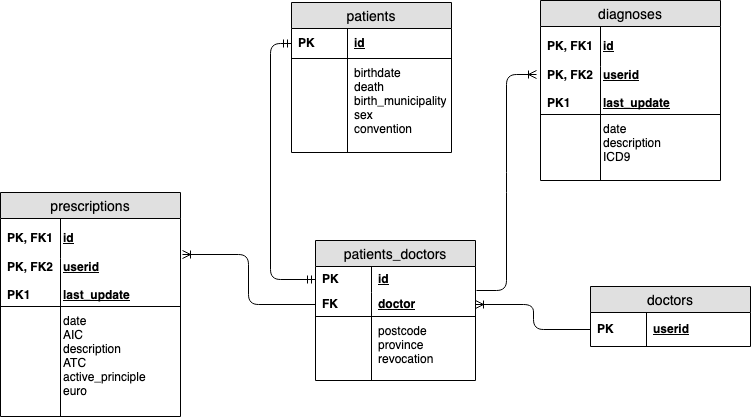
\includegraphics[scale=0.58]{images/er.png}
	\caption{\small ER model}
	\label{er}
\end{figure}

\section[Preliminary analysis]{Example of preliminary analysis}
Analysis on patients' gender, on 1 015 618 distinct patients, with approx. percentages:
\begin{itemize}
	\item Males: 479 556, 47\%;
	\item Females: 533 256, 52\%;
	\item Other or null, 2 806,  < 1\%.
\end{itemize}

Percentages of males and females are coherent with ISTAT data of 2018, showing 48\% males and 52\% females in the whole region Campania\footnote{\href{http://demo.istat.it/bil2018/index.html}{ISTAT 2018}}, confirming the validity of data.

The 1\% of missing data introduces the \textbf{information loss} issue, which will be examined in detail in the next part of the research.

\subsection{Variations through time}
To give a general idea on variations of available information and magnitude orders, a \textbf{snapshot} of 2010-2017 is used to show patterns and differences.

It is expected for data to progressively increase, since more and more general practitioners have familiarised with the electronic recording systems within years.

A first analytical approach consists in counting the number of patients getting at least a diagnosis for each year:
\begin{table}[h]
	\centering
	 \makebox[\textwidth][c]{
	\begin{tabular}{c|c|c|c|c|c|c|c|c}
		  & \textbf{2010} & \textbf{2011} & \textbf{2012} & \textbf{2013} & \textbf{2014} & \textbf{2015} & \textbf{2016} & \textbf{2017} \\
		\hline
		\textbf{Patients} & 329 715 & 320 253 & 316 431 & 320 948 & 324 920 & 323 441 & 330 641 & 326 987 \\
		\hline
		\textbf{Age mean} & 47,43 & 47,89 & 48,44 & 48,68 & 48,98 & 49,78 & 50,12 & 50,54 \\
		\hline
		\textbf{Age s.\ d.} & 20,7 & 20,81 & 20,84 & 20,86 & 20,87 & 20,84 & 20,85 & 20,79 \\
		\hline
		\textbf{Women} & 185 035 & 179 700 & 178 248 & 180 304 & 182 286 & 181 313 & 185 729 & 183 419 \\
		\hline
		\textbf{Men} & 144 016 & 140 330 & 137 514 & 139 780 & 141 727 & 141 158 & 143 931 & 142 363 \\
	\end{tabular}}
\caption{\small Number of patients with diagnoses}
\vspace{-10px}
\end{table}
\bigskip

Another example can be obtained counting the number of prescriptions each year:
\begin{table}[h]
	\centering
	 \makebox[\textwidth][c]{
	\begin{tabular}{c|c|c|c|c|c|c|c|c}
		& \textbf{2010} & \textbf{2011} & \textbf{2012} & \textbf{2013} & \textbf{2014} & \textbf{2015} & \textbf{2016} & \textbf{2017} \\
		\hline
		\textbf{P.} & 7 326 923 & 7 108 288 & 7 269 855 & 7 541 539 & 7 777 753 & 7 847 313 & 7 856 246 & 7 785 325 \\
	\end{tabular}}
\caption{\small Number of patients with prescriptions}
\end{table}

Patients getting diagnoses tend to remain stable, yet prescriptions have a difference of more than 450 000 records, confirming the hypothesis of information registering increase while raising the concern of an effective general overprescribing.
